\documentclass{llncs}

\usepackage{epsfig}
\usepackage{graphicx}
\usepackage{color}
\usepackage{amsfonts}
\usepackage{amsmath}
\usepackage{mathabx}
%\usepackage{hyperref}
%\usepackage{subfigure}
%\usepackage[colorinlistoftodos, textwidth=3.2cm, shadow]{todonotes}

\usepackage{algorithm}
\usepackage{fixltx2e}
\usepackage{algpseudocode}

\usepackage{multirow}

% To use Call inside another Call (algorithms)
\MakeRobust{\Call}


%%%%%%%%%%%%%%%%%%%%%%%%%%%%%%%%%%%%%%%%%%
%
% Title
%
%%%%%%%%%%%%%%%%%%%%%%%%%%%%%%%%%%%%%%%%%%
\title{RTS AI: Problems and Techniques
%\thanks{Supported by ...}
}

\author{Santiago~Onta\~{n}\'{o}n\inst{1} \and 
		Gabriel~Synnaeve\inst{2} \and
		Alberto~Uriarte\inst{1} \and
		Florian~Richoux\inst{3} \and
		David~Churchill\inst{4} \and
		Mike~Preuss\inst{5}
		}

\institute{
	Computer Science Department at Drexel University, Philadelphia, PA, USA. \\
	\email{\{santi,albertouri\}@cs.drexel.edu}
\and
	Cognitive Science and Psycholinguistics (LSCP) of ENS Ulm, Paris, France. \\
	\email{gabriel.synnaeve@gmail.com}
\and
	Nantes Atlantic Computer Science Laboratory (LINA), Univ. Nantes, France.\\
	\email{florian.richoux@univ-nantes.fr}
\and
	Computing Science Department of the University of Alberta, Edmonton, Canada. \\
	\email{cdavid@cs.ualberta.ca}
\and
	Department of Computer Science of Technische Universit{\"a}t Dortmund, Germany.
	\email{mike.preuss@cs.tu-dortmund.de}
}

\begin{document}

\maketitle

%\begin{abstract}
%  This is the abstract.
%\end{abstract}

\section*{Synonyms}

Real-Time Strategy games; RTS games; Artificial Intelligence; AI; Game AI

\section*{Definition}

{\em Real-Time Strategy} (RTS) games  is a sub-genre of strategy games
where  players  need to  build  an  economy (gathering  resources  and
building a  base) and military  power (training units  and researching
technologies)  in order  to defeat  their opponents  (destroying their
army and base).  Artificial Intelligence problems related to RTS games
deal with  the behavior of  an artificial player. This  consists among
others to learn  how to play, to have an  understanding about the game
and  its environment,  to predict  and  infer game  situations from  a
context and sparse information.

\section*{Introduction}\label{sec:intro}
The  field of  Real-Time Strategy  (RTS) game  Artificial Intelligence
(AI) has advanced significantly in the past few years, partially thanks to competitions as the ``ORTS
RTS  Game AI  Competition''  (held  from 2006  to  2009), the  ``AIIDE
StarCraft AI Competition'' (held since  2010), and the ``CIG StarCraft
RTS AI Competition'' (held since  2011). Based on the work work presented in \cite{ontanon2013survey}, here we first define RTS games, then list the open problems in creating AI for RTS games, and finally point to the approaches that have been proposed to address these problems.

%Complex  dynamic  environments,  where neither  perfect  nor  complete
%information  about the  current state  or  about the  dynamics of  the
%environment are available, pose  significant challenges for artificial
%intelligence. Road traffic, finance, or weather forecasts are examples
%of such large, complex, real-life  dynamic environments. RTS games can
%be seen  as a simplification  of one such real-life  environments, with
%simpler dynamics in a finite and smaller world, although still complex
%enough to  study some  of the key  interesting problems  like decision
%making under  uncertainty or  real-time adversarial  planning. Finding
%efficient techniques for tackling these problems on RTS games can thus
%benefit other  AI disciplines and  application domains, and  also have
%concrete and direct applications in the ever growing industry of video
%games.

% Some other arguments for the motivation: 
% 1. It's fun 
% 2. Togelius' argument: Some problems  are very similar than the ones
% in  robotics (decision  making, pathfinding,  ...).  However  RTS AI
% does  not have  the same  limitations for  running experiments:  few
% hardware constraints (we just need  a computer), we can have control
% on the time flow, we can run many experiments in parallel, ...


%This article aims to  provide an overview on what is  the state of the
%art  in  RTS AI,  with  a  particular emphasis  on  the  work done  in
%StarCraft.  It is organized as follows: 
%{\color{blue} TODO (or not)}

% Section~\ref{sec:rts}
% introduces RTS games, in particular the game StarCraft, and their main
% AI challenges.  Section~\ref{sec:review} reviews  the existing work on
% tackling  these   challenges  in  RTS   games.   Section~\ref{sec:bot}
% analyzes  several current  state of  the art  RTS game  playing agents
% (called  {\em  bots}),  selected   from  the  participants  to  annual
% StarCraft  AI  competitions.   Section~\ref{sec:competition}  presents
% results of  the recent annual competitions  held at the AIIDE  and CIG
% conferences  and  a  StarCraft bot  game  ladder\footnote{An  extended
%   tournament,   which   can    potentially   go   on   indefinitely.}.
% Section~\ref{sec:questions}  compiles  open   questions  in  RTS  game
% AI. Finally, the paper concludes on discussions and perspectives.


\section*{Real-Time Strategy Games}\label{sec:rts}

From a  theoretical point  of view, the  main differences  between RTS
games and traditional board games such as Chess are:

\begin{itemize}
\item  RTS games are  {\em simultaneous  move} games,  where more than one
  player  can issue  actions  at the  same  time. 
\item Action in RTS games are {\em durative}, i.e.  actions are not instantaneous, but
  take some amount of time to complete.
\item RTS games  are ``real-time'', which actually means is that each
  player  has  a  very  small  amount  of  time  to  decide  the  next
  move, and that, in contrast to {\em turn-based} games, the game keeps advancing even if a player does not execute any actions. Compared to  Chess, where players may have several minutes to
  decide the next action, in StarCraft, a popular RTS game, the game executes at 24 frames
  per second, which means that players  can act as fast as every 42ms,
  before the game state changes.
\item Most  RTS games are  partially observable: players can  only see
  the part of the  map that has been explored. This  is referred to as
  the {\em fog-of-war}.
\item Most RTS games are non-deterministic: some actions have a chance
  of success, and the amount of damage dealt by different units is sometimes stochastic.
\item And  finally, the complexity  of these  games, both in  terms of
  state space size and in terms of number of actions available at each
  decision cycle is very large. For  example, the state space of Chess
  is typically  estimated to  be around  $10^{50}$, heads  up no-limit
  Texas holdem  poker around $10^{80}$,  and Go around  $10^{170}$. In
  comparison,  the  state space  of  StarCraft  in  a typical  map  is
  estimated to be  many orders of magnitude larger than  any of those,
  as discussed in the next section.
\end{itemize}

For those reasons, standard techniques  used for playing classic board
games, such as  game tree search, cannot be directly  applied to solve
RTS games without the definition of some level of abstraction, or some
other simplification. Interestingly enough, humans  seem to be able to
deal with the  complexity of RTS games, and are  still vastly superior
to       computers      in       these       types      of       games
\cite{burochurchill2012aimagazine}.   For  those   reasons,  a   large
spectrum of techniques  have been attempted to deal  with this domain,
as we will describe below. 
%The remainder of this section is devoted to describe StarCraft  as a research  testbed, and on detailing  the open
% challenges in RTS game AI.


%\subsection{StarCraft}\label{subsec:StarCraft}
%{\color{blue}  Do we  need this  part?  Should  we talk  about RTS  AI
%  problems  and   techniques  in  general,  but   take  examples  from
%  StarCraft only, arguing this game is mainstream?}
In the past few years, {\em StarCraft: Brood War} (an immensely popular  
RTS game released in 1998 by Blizzard  Entertainment) has become the 
standard testbed for evaluating AI techniques in RTS games.
%{\em StarCraft: Brood  War} is an immensely popular  RTS game released
%in   1998  by   Blizzard  Entertainment.   
StarCraft  is   set  in   a
science-fiction based universe where the player must choose one of the
three  races: Terran,  Protoss or  Zerg.  %One of  the most  remarkable
%aspects  of StarCraft  is  that  the three  races  are extremely  well
%balanced.
%
% \begin{itemize}
% \item Terrans provide  units that are versatile and  flexible giving a
%   balanced option between Protoss and Zergs.
% \item  Protoss   units  have   lengthy  and   expensive  manufacturing
%   processes, but they are strong and resistant.  These conditions make
%   players follow a strategy of quality over quantity.
% \item Zergs, the insectoid race, units are cheap and weak. They can be
%   produced fast, encouraging players to overwhelm their opponents with
%   sheer numbers.
% \end{itemize}
%
% What about copyright problems with this screenshot?
% Figure~\ref{fig:StarCraft} shows  a screenshot of StarCraft  showing a
% player playing the Terran race.
%
%{\color{blue}  Thus,  merge the  following  paragraph  with the  first
%  paragraph of the RTS section?}
In order to win a StarCraft  game, players must first gather resources
(minerals  and Vespene  gas). As  resources become  available, players
need to allocate them for creating more buildings (which reinforce the
economy, and allow players to  create units or unlock stronger units),
research  new technologies  (in order  to  use new  unit abilities  or
improve the units)  and train attack units. Units  must be distributed
to  accomplish different  tasks  such as  reconnaissance, defense  and
attack.  While  performing all  of those tasks,  players also  need to
strategically understand the geometry of the  map at hand, in order to
decide where to place new buildings  (concentrate in a single area, or
expand  to  different  areas)  or where  to  set  defensive  outposts.
Finally, when  offensive units of  two players meet, each  player must
quickly maneuver each  of the units in order to  fight a battle, which
requires quick and reactive control of each of the units.

% \begin{figure}
%     \centering
%     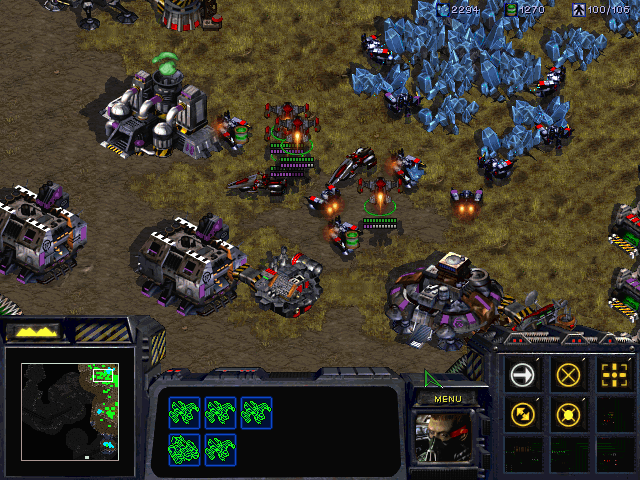
\includegraphics[width=0.8\columnwidth]{figures/starcraft1.png}
%     \caption{A screenshot of \emph{StarCraft: Brood War}.}
%     \label{fig:StarCraft}
% \end{figure}

% A typical  StarCraft map is defined  as a rectangular grid,  where the
% $width \times  height$ of  the map  is measured in  the number  of $32
% \times 32$ squares of pixels, also  known as build tiles. However, the
% resolution of  walkable areas is  in squares  of $8 \times  8$ pixels,
% also known as  walk tiles. The typical dimensions for  maps range from
% $64  \times 64$  to  $256 \times  256$ build  tiles.  Each player  can
% control  up to  200 units  (plus  an unlimited  number of  buildings).
% Moreover,  each different  race contains  between 30  to 35  different
% types of units  and buildings, most of them with  a significant number
% of  special abilities.  All these  factors together  make StarCraft  a
% significant  challenge, in  which humans  are still  much better  than
% computers.      For     instance,      in     the      game     ladder
% iCCup\footnote{http://www.iccup.com/StarCraft/} where users are ranked
% by their current point totals ($E$ being the lowest possible rank, and
% $A^+$  and  $Olympic$ being  the  second  highest and  highest  ranks,
% respectively), the best  StarCraft AI bots are ranked  between $D$ and
% $D^+$,  where average  amateur players  are ranked  between $C^+$  and
% $B$. For comparison, StarCraft professional players are usually ranked
% between $A^-$ and $A^+$.

From a theoretical point of view,  the state space of a StarCraft game
for a  given map is  enormous.  For  example, consider a  typical $128
\times 128$ map. At any given moment  there might be between 50 to 400
units in  the map, each of  which might have a  complex internal state
(remaining energy  and hit-points, action being  executed, etc.). This
quickly leads to an immense number  of possible states (way beyond the
size  of smaller  games,  such  as Chess  or  Go).  For example,  just
considering the location of each  unit (with $128 \times 128$ possible
positions per  unit), and  400 units,  gives us  an initial  number of
$16384^{400} \approx 10^{1685}$. If we add the other factors playing a
role in the game, such as resources, hit-points, energy, research status, cool-down timers, etc., we obtain even larger numbers (see \cite{ontanon2013survey} for a more in-depth description of the complexity of StarCraft).

% Another way to measure the complexity of the game is by looking at the
% branching factor,  $b$, and the  depth of  the game, $d$,  as proposed
% in~\cite{Gaby}, with  a total game  complexity of $b^d$. In  Chess, $b
% \approx 35$  and $d \approx  80$. In more  complex games, like  Go, $b
% \approx  30$ to  $300$, and  $d  \approx 150$  to $200$.  In order  to
% determine the  branching factor in StarCraft  when an AI plays  it, we
% must have in mind, that the  AI can issue actions simultaneously to as
% many  units in  the  game as  desired. Thus,  considering  that, in  a
% typical game, a player controls between 50 to 200 units, the branching
% factor  would be  between $u^{50}$  and  $u^{200}$, where  $u$ is  the
% average number of actions each unit can execute.  Estimating the value
% of $u$ is not easy, since the  number of actions a unit can execute is
% highly  dependent   on  the  context.   Let  us  make   the  following
% assumptions: 1) at most 16 enemy units  will be in range of a friendly
% unit (larger values  are possible, but unlikely), 2) when  an AI plays
% StarCraft, it only makes sense to  consider movement in the 8 cardinal
% directions per unit  (instead of assuming that the player  can issue a
% ``move'' command to anywhere in the map  at any point in time), 3) for
% ``build'' actions,  we consider that  SCVs (Terran worker  units) only
% build in their  current location (otherwise, if they need  to move, we
% consider  that  as  first  issuing  a  ``move''  action,  and  then  a
% ``build''), and  4) let's  consider only the  {\em Terran}  race. With
% those assumptions,  units in  StarCraft can  execute between  1 (units
% like ``Supply  Depots'', whose only  action is  to be ``idle'')  to 43
% actions (Terran ``Ghosts''), with typical values around 20 to 30. Now,
% if we have in mind that actions have cool-down times, and thus not all
% units can  execute all of  the actions at every  frame, we can  take a
% conservative estimation  of about $10$  possible actions per  unit per
% game frame. This results in  a conservative estimate for the branching
% factor  between $b  \in  [10^{50},10^{200}]$,  only considering  units
% (ignoring the actions buildings can execute).

% Assuming  a conservative  value for  $u$  of about  $30$ (moving  to
% nearby positions, attacking units in range, using special abilities,
% etc.), we  obtain a  branching factor of  $b$ between  $30^{50}$ and
% $30^{200}$.

% Now, to  compute $d$, we simply  consider the fact that  typical games
% last for  about 25  minutes, which  results in  $d \approx  36000$ (25
% minutes $\times$ 60 seconds $\times$ 24 frames per second).


% In StarCraft,  humans can issue only  one action at a  time (this is
% because of  the GUI  used by  the game,  computer players  can issue
% several  actions, to  different  units, at  any  given time),  thus,
% assuming a  player controls between 50  to 200 units, and  that each
% unit can execute  between 4 to 20  actions (moving in each  of the 4
% cardinal  directions,   attacking  units   in  range,   use  special
% abilities, etc.), we estimate the branching factor for human players
% to be around $b \approx 200  - 4000$. Good players can execute about
% 300 actions per minute, and the typical length of a game is about 25
% minutes. Thus, $d \approx 7500$.

% However, this  is a weak indication  of the complexity of  the game,
% since many  of those states  would never be  reached in a  game. For
% that  reason, it  is  more useful  to  just think  in  terms of  the
% branching factor  and depth  of a  game, when a  human plays  it. In
% Chess,  the branching  factor is  around  35 and  the depth,  around
% 80. In Go, the  branching factor is between 30 to  300 and the depth
% 150 to 200. In StarCraft, humans can execute about ...


% From Gabriel's dissertation:
% ------------------------------------
%How does the state of possible actions grow? To measure this, we
%used a measure from perfect information zero-sum games (as Checkers,
%Chess and Go): the branching factor* b and the depth d of a typical
%game. The complexity of a game (for taking a decision) is proportional
%to bd.
%[...]
%In RTS games, b = 200 is a lower bound (in StarCraft we may have
%between 50 to 400 units to control), and very good amateurs and
%professional players perform more than 300 actions per minute. As
%StarCraft is a simultaneous move, multi-units game, a strict number
%for b would be |actions||units| (actions account for atomic moves and
%abilities), thus for StarCraft b would be around 30^{60}. Strictly
%speaking, for a StarCraft game, d = 24  game_seconds (24 game frames
%per second), with a game duration of 25 minutes, this gives d =
%36,000, thus b^d Å% 30^{60^{36000}} .
%I

\section*{Challenges in RTS Game AI}\label{subsec:challenges}

Early research  in AI  for RTS  games \cite{Buro03rts}  identified the
following six challenges: Resource management, Decision making under uncertainty, Spatial and temporal reasoning, Collaboration (between multiple AIs), Opponent modeling and learning, and Adversarial real-time planning. While there  has been  a significant  work in  many, others  have been
untouched (e.g. collaboration). Moreover, recent research in this area
has identified several additional research  challenges, such as how to
exploit the massive amounts  of existing domain knowledge (strategies,
build-orders,  replays,  and  so   on). Thus, the challenges in RTS game AI can be grouped in six main different areas, described below.

%\begin{itemize}
%\item Task Decomposition (or ``Architecture'')
%\item Integration of Domain Knowledge
%\item Reasoning with Uncertainty (including information gathering)
%\item Opponent Modeling  and Adaptation: opponent modeling  is key if
%  we  have  to  adapt  our  strategy.  As  different  strategies  are
%  dominating each  others, forming  multiple Nash equilibria,  the AI
%  has to be able to infer the intend of its opponent.
%\item  Group   and  Individual  Control  (``micro''):   the  task  of
%  controlling units efficiently (we can  not speak of optimality here
%  due to  the huge  state space,  and of  the enemy  behavior entails
%  numerous  Nash  equilibria),  focusing  fire  to  diminish  enemy's
%  firepower  and  keeping  our   units  alive  the  longest,  casting
%  defensive and offensive spells and abilities.
%\item Planning and Resource Allocation (``macro'')
%\item Spatial reasoning (``tactics'')
%\end{itemize}

\subsubsection{Planning}
As mentioned above, the  size of the state space in  RTS games is much
larger  than  that  of  traditional  board  games  such  as  Chess  or
Go. Additionally,  the number  of actions  that can  be executed  at a
given instant of time is  also much larger. Thus, standard adversarial
planning  approaches,  such  as  game tree  search  are  not  directly
applicable. As we  elaborate later, planning in RTS games  can be seen
as having multiple  levels of abstraction: at a  higher level, players
need long-term  planning capabilities,  in order  to develop  a strong
economy in the game; at a low level, individual units need to be moved
in coordination to  fight battles taking into account  the terrain and
the  opponent.  Techniques  that  can  address  these  large  planning
problems by either sampling, or  hierarchical decomposition do not yet
exist.

\subsubsection{Learning}
Given  the  difficulties  in  playing  by  directly  using
adversarial  planning techniques,  many  research  groups have  turned
attention to  learning techniques. We  can distinguish three  types of
learning problems in RTS games:
\begin{itemize}
\item {\em Prior learning}: How can we exploit available data, such as
  existing replays,  or information  about specific maps  for learning
  appropriate strategies before hand? A significant amount of work has
  gone in this
  direction.%, such as \cite{WeberCIG09,SynnaeveCIG11,SynnaeveAIIDE11,OntanonMSR10}.
\item  {\em In-game  learning}: How  can bots  deploy online  learning
  techniques that allow them to  improve their game play while playing
  a  game?  These  techniques  might  include  reinforcement  learning
  techniques, but  also opponent modeling.  The main problem  again is
  the fact  that the state  space is too large  and the fact  that RTS
  games are partially observable.
\item {\em  Inter-game learning}:  What can be  learned from  one game
  that can  be used  to increase  the chances of  victory in  the next
  game? Some work has used simple game-theoretical solutions to select
  amongst a  pool of  predefined strategies,  but the  general problem
  remains unsolved.
\end{itemize}

%%% I  think there  are two  important aspects  of uncertainty  in RTS
%%% games:
%%% \begin{itemize}
%%% \item First  is trying to model  uncertainty and try to  reduce it
%%%   (information gathering,  and representation of  knowledge), this
%%%   includes scouting,  and maintaining good estimates  of locations
%%%   and number of units of the enemy, etc.
%%% \item Second  is actually using the  uncertain information. Taking
%%%   decisions  like  army strength  estimation  (like  to attack  or
%%%   retreat).
%%% \end{itemize}

\subsubsection{Uncertainty}
Adversarial planning under  uncertainty in domains of the  size of RTS
games is  still an unsolved  challenge.  In  RTS games, there  are two
main kinds  of uncertainty. First,  the game is  partially observable,
and players  cannot observe the  whole game  map (like in  Chess), but
need to scout in order to see what the opponent is doing. This type of
uncertainty   can  be   lowered  by   good  scouting,   and  knowledge
representation  (to  infer  what  is  possible  given  what  has  been
seen). However, scouting also means deliberately reducing economic progress in order to obtain information.
Second,  there is also  uncertainty arising from the  fact that
the games  are adversarial,  and a player  cannot predict  the actions
that the opponent(s)  will execute. For this type  of uncertainty, the
AI, as the human  player, can only build a sensible  model of what the
opponent is likely to do.
% [Santi:  I  commented  out  this  part,  since  I'm  not  sure  it's
% correct.  The second  type  of  uncertainty can  also  be linked  to
% data.  For example,  by analyzing  player replays,  one could  learn
% "plan recognition"  probability tables, which  can be used  to infer
% the strategy  of the opponent,  and thus, reduce the  uncertainty of
% the opponent's future  actions] Both these kinds  of uncertainty can
% be studied through probabilities, but only the first type, $P(Hidden
% | Seen)$, can be {\em easily} linked to
% data. %now for the clumsy part:
% One could  argue that the  extensional data  is the only  thing that
% matters because  it is the only  thing that has an  influence on the
% game, but in  reality, for very highly  skilled players, discovering
% the intentions of the  enemy is the key to winning.  It allows for a
% compact understanding of the game  state and development, while also
% giving additional information about the  future. Whereas a player is
% doing action  A to  follow it  up by action  B or  C depends  on its
% intention,  while the  information  about action  A  is visible  and
% information about  B or  C is  hidden, only  intention allows  for a
% choice.

\subsubsection{Spatial and Temporal Reasoning}
% TODO just a paragraph on exposing why there are temporal and spatial
% reasoning in RTS AI.
Spatial reasoning is  related to each aspect  of terrain exploitation.
It  is  involved   in  tasks  such  as  building   placement  or  base
expansion.  In the  former,  the player  needs  to carefully  consider
building  positioning into  its  own  bases to  both  protect them  by
creating  defenses or walls  against invasions  and to  avoid bad  configurations
where large units could be stuck. In base expansion, the player has to
choose good available locations to build a new base, regarding its own
position and  opponent's bases. Finally,  spatial reasoning is  key to
tactical reasoning:  players need to  decide where to place  units for
battle, favoring, for instance,  engagements when the opponent's units
are lead into a bottleneck.

% [Flo:  70% to hit high  ground units according to  Ben Weber's paper
% [3], and 53.125% according  to BWAPI website. Who's right? Should we
% add this in the paper?]

% [Alberto: I  guess Weber's number comes  from StarCraft walkthroughs
% like                                                           this:
% http://www.supercheats.com/pc/walkthroughs/starcraftbroodwar-walkthrough01.txt,
% there is also a chance to hit in even grounds (like
% 98%). But since we cannot see the original code all of these numbers are approximations. In any case we can keep explaining the concept without numbers ;)]
%Another example of spatial reasoning in StarCraft is that it is always
%an advantage to  have own units on  high ground while the  enemy is on
%low ground,  since units on  low ground have  no vision onto  the high
%ground. %, and firing from low ground have a chance to hit units on high ground.
%MP: took out last half sentence as it seems to be rather confusing.

Analogously,  temporal  reasoning  is  key in  tactical  or  strategic
reasoning.  For  example,  timing  attacks and  retreats  to  gain  an
advantage. At a  higher strategic level, players need  to reason about
when to  perform long-term impact  economic actions such  as upgrades,
building  construction,  strategy  switching,  etc.  all  taking  into
account  that the  effects of  these  actions are  not immediate,  but
longer term.


\subsubsection{Domain Knowledge Exploitation}
In traditional board  games such as Chess,  researchers have exploited
the  large  amounts  of  existing  domain  knowledge  to  create  good
evaluation  functions  to be  used  by  alpha-beta search  algorithms,
extensive opening books, or end-game tables. In the case of RTS games,
it  is still  unclear how  the  significantly large  amount of  domain
knowledge  (in the  forms or  strategy guides,  replays, etc.)  can be
exploited. Most  work in  this area has  focused on  two main
directions: (1) hard-coding existing strategies into bots (so that  bots only  need to
decide  which strategies  to deploy,  instead of  having to  solve the
complete  planning problem), and (2) mining large datasets
of  replays \cite{WeberCig09,synnaeve2012dataset} to automatically extract
 strategies,  trends   or  plans. % However,  StarCraft  games  are  quite  complex,  and  how  to
%automatically learn from such datasets is still an open problem.

\subsubsection{Task Decomposition}
Most existing approaches  to play RTS games work by decomposing the  problem into   a    collection   of    smaller   problems to    be   solved
independently. Specifically, a common subdivision is:
\begin{itemize}
\item {\em  Strategy}: corresponds  to the high-level  decision making
  process.  This is  the highest  level  of abstraction  for the  game
  comprehension.  Finding an  efficient  strategy or  counter-strategy
  against a given opponent is key in RTS games, and concerns the whole
  set of units a player
  owns. %If we may allow ourselves a military analogy, strategy is orders given by generals at the HQ.
\item   {\em  Tactics}:   are  the   implementation  of   the  current
  strategy.  It  implies  army and  building  positioning,  movements,
  timing, and so on. Tactics concerns a group of
  units. %They are orders given by officers on the battlefield.
\item {\em Reactive  control}: is the implementation  of tactics. This
  consists   in  moving,   targeting,  firing,   fleeing,  hit-and-run
  techniques  (also  knows  as  ``kiting'')  during  battle.  Reactive
  control focuses on a specific
  unit. %It is soldiers applying officers' orders.
%\end{itemize}
%
%\noindent
%Both  strategy  and  tactics  are  usually  called
%\textit{macro-management}, whereas reactive control is also called
%\textit{micro-management}. In addition of the three tasks shown above,
%one could also consider these two tasks that an AI has to deal with:
%\begin{itemize}
\item  {\em Terrain  analysis}: consists  in the  analysis of  regions
  composing the map: choke-points,  minerals and gas emplacements, low
  and high walkable grounds, islands, etc.
\item  {\em   Intelligence  gathering}:  corresponds   to  information
  collected  about the  opponent. Because  of the  fog-of-war, players
  must regularly send scouts to localize and spy enemy
  bases.%, and must see or infer what buildings and technology the enemy has developed in order to adapt its strategy.
\end{itemize}

In comparison, when humans play StarCraft, they typically divide their
decision  making in  a  very different  way.  The StarCraft  community
typically talks about two tasks:
\begin{itemize}
\item  {\em  Micro}: is  the  ability  to control  units  individually
  (roughly corresponding to {\em Reactive  Control} above, and part of
  {\em Tactics}). A good \emph{micro} player usually keeps their units
  alive over a longer period of time.
\item {\em  Macro}: is the ability  to produce units and  to expand at
  the  appropriate times  to  keep your  production  of units  flowing
  (roughly corresponding to everything  but {\em Reactive Control} and
  part of {\em Tactics} above). A good \emph{macro} player usually has
  the larger army.
\end{itemize}

The reader can find a good  presentation of task decomposition RTS game AI in~\cite{weber2011acs}.  Although  the   previous  task decomposition  is  common, other task decompositions have been explored (see \cite{ontanon2013survey} for an overview of the task decomposition used by several StarCraft bots).



\section*{Existing work on RTS Game AI}\label{sec:review}

\begin{figure}
    \centering
%    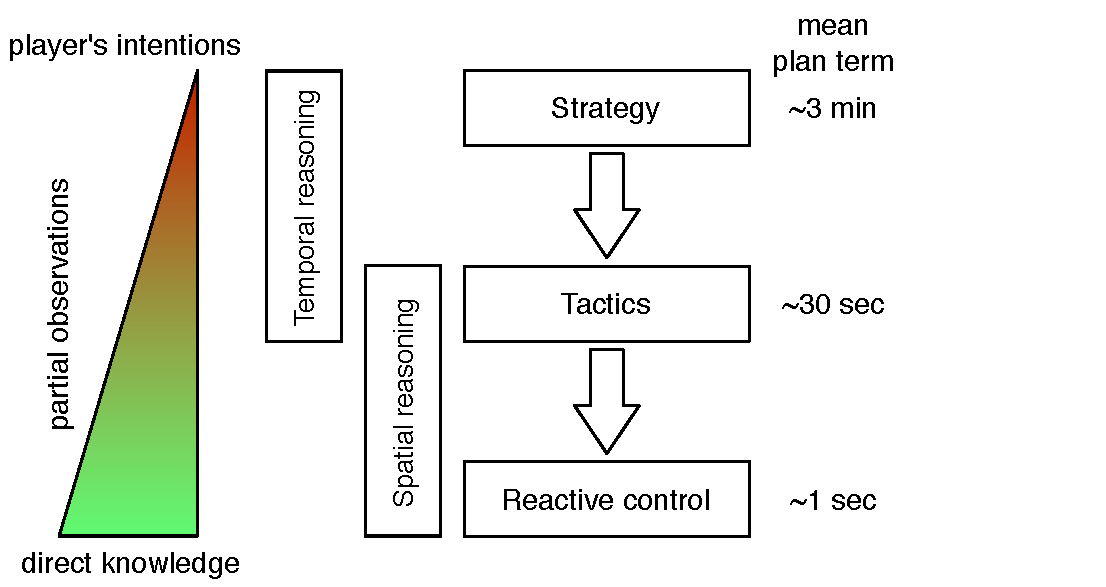
\includegraphics[width=0.7\columnwidth]{figures/levels_abstraction.pdf}
    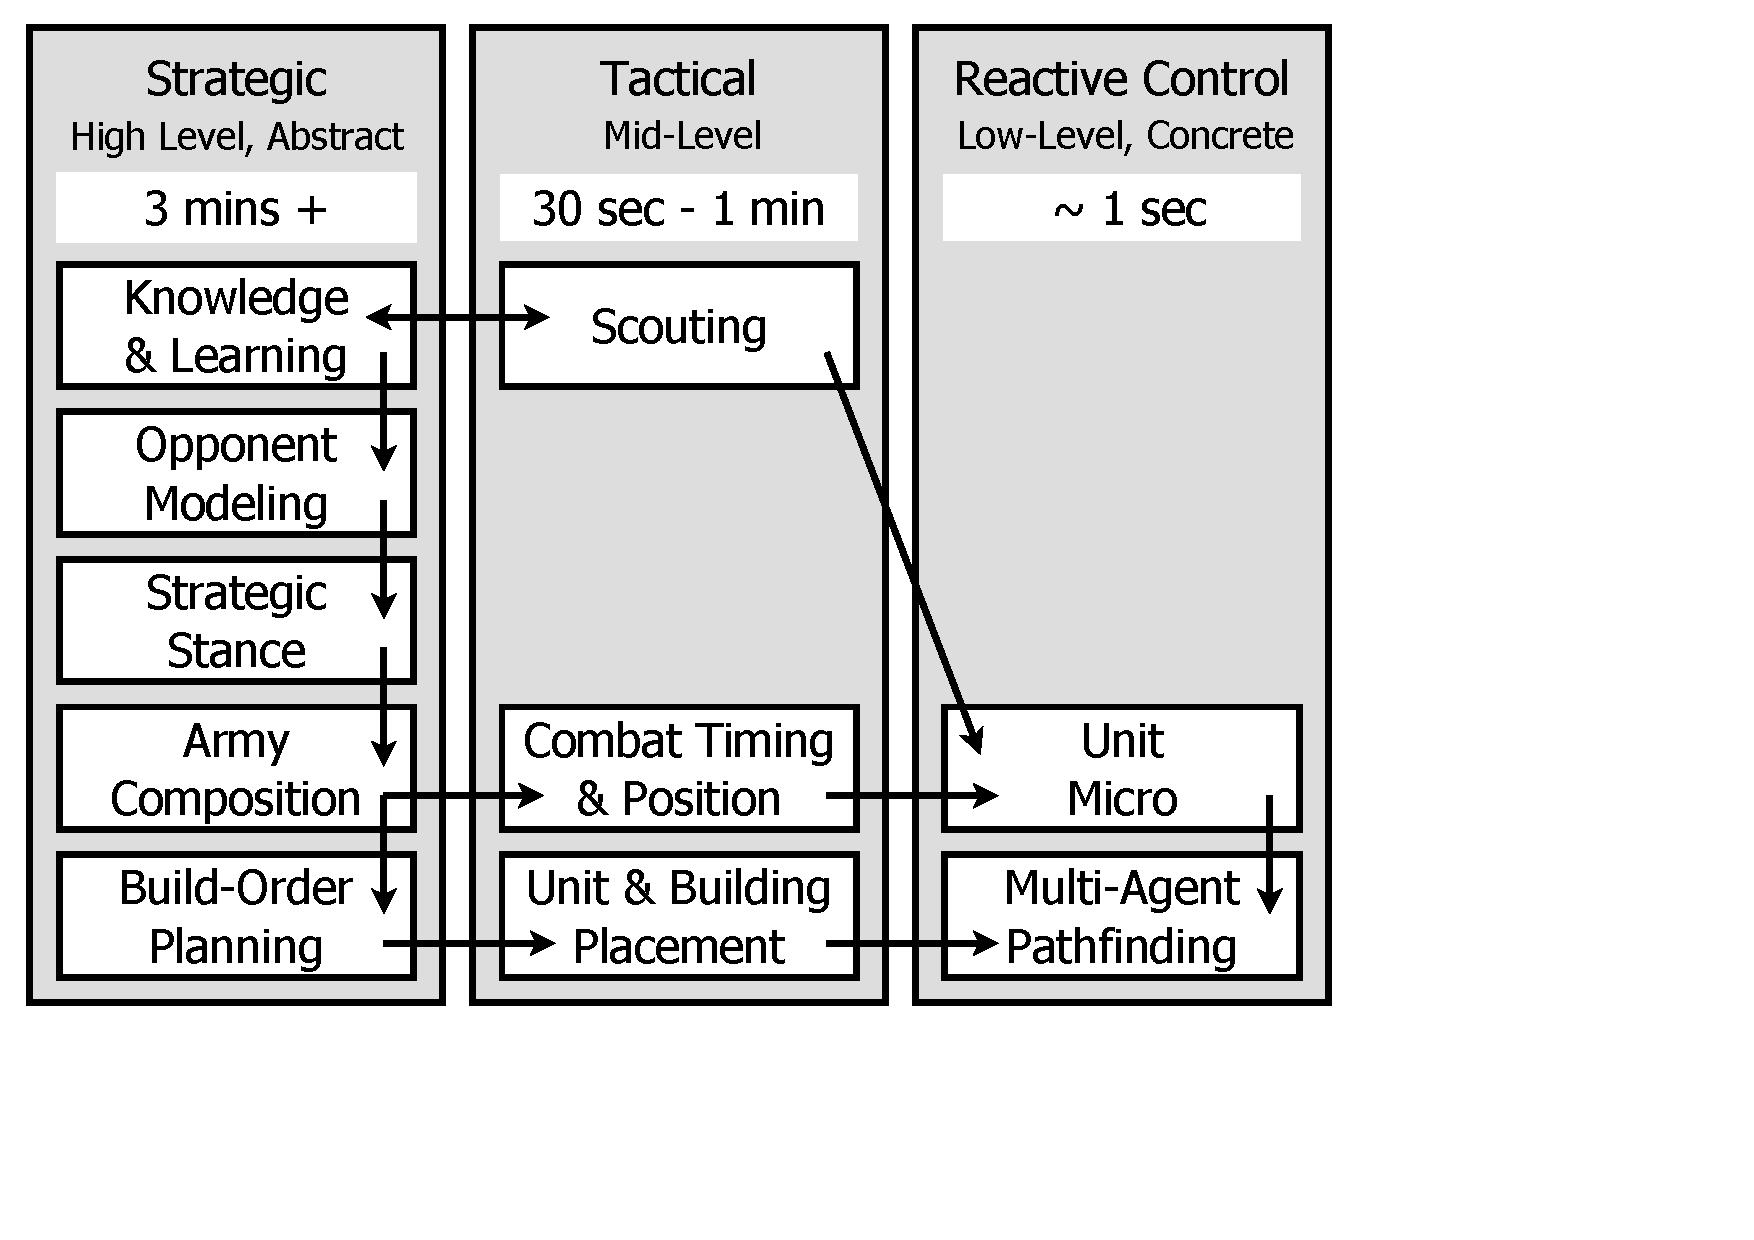
\includegraphics[width=0.7\columnwidth]{figures/categories}
    \caption{RTS  AI  levels  of abstraction  and  typical sub-problems associated with them:
      %uncertainty  (coming  from  partial  observation  and  from  not knowing the  intentions of  the opponent)  is higher  for higher abstraction  levels.  
      Timings correspond  to  an
      estimate   of   the   duration   of   a   behavior   switch   in
      StarCraft. %Spatial and temporal  reasoning are indicated for the levels at which greedy solutions are not enough.
      }
    \label{fig:levels-abstraction}
\end{figure}

Systems that  play RTS  games need  to address most,  if not  all, the
aforementioned problems  together. Therefore,  it is hard  to classify
existing  work  on  RTS  AI   as  addressing  the  different  problems
above. For that reason, %in order to classify existing work on RTS AI,
we will divide  it according to three levels  of abstraction: strategy
(which loosely corresponds to ``macro''), tactics, and reactive control
(which loosely corresponds to ``micro'').

Figure~\ref{fig:levels-abstraction}   illustrates   how
strategy, tactics, and reactive control are three points in a continuum
scale where  strategy corresponds  to decisions making  processes that
affect long spans of time (several  minutes in the case of StarCraft),
reactive control corresponds  to low-level second-by-second decisions,
and tactics sit in the  middle. Also, strategic decisions reason about
the whole game at once, whereas tactical or reactive control decisions
are localized,  and affect only  specific groups of  units. Typically,
strategic decisions constrain future tactical decisions, which in turn
condition  reactive  control.  Moreover,  information  gathered  while
performing reactive control, can  cause reconsideration of the tactics
being employed; which could trigger further strategic reasoning.

The remainder of this section presents work toward addressing the previous six open RTS game AI problems, grouped as work focused toward strategy, tactics, or reactive control, as well as a final section dedicated to holistic approaches that attempt to deal with all three levels at once.

%Following this idea, we consider  strategy to be everything related to
%the  technology trees,  build-order\footnote{The {\em  build-order} is
%  the specific sequence in which  buildings of different types will be
%  constructed at  the beginning of  a game, and  completely determines
%  the   long-term  strategy   of  a   player.},  upgrades,   and  army
%composition. It  is the most  deliberative level, as a  player selects
%and performs  a strategy  with future stances  (aggressive, defensive,
%economy, technology)  and tactics in  mind. We consider tactics  to be
%everything related to confrontations between groups of units. Tactical
%reasoning involves both spatial  (exploiting the terrain) and temporal
%(army  movements)  reasoning, constrained  on  the  possible types  of
%attacks   by  the   army   composition  of   the   player  and   their
%opponent. Finally, reactive control  describes how the player controls
%individual units to  maximize their efficiency in  real-time. The main
%difference  between  tactics and  reactive  control  is that  tactical
%reasoning  typically involves  some sort  of planning  ahead for  some
%short spans  of time,  whereas reactive  control involves  no planning
%ahead whatsoever.

% Example:
%For example,  after starting a  game, a player  might decide to  use a
%{\em rushing}  strategy (which involves  quickly building an  army and
%sending it  to attack as  early as possible  in the game);  then, when
%performing the attack use a {\em surrounding} tactic, where the player
%tries to surround the enemy  cutting potential escape routes; finally,
%while executing the surrounding tactic, the player might decide to use
%reactive control  techniques that command individual  units to perform
%repeated {\em attack  and flee} movements, to  maximize the efficiency
%of each of the units being used in the attack.

% {\color{blue}  perhaps  TODO  ``how  it's  done  in  the  industry''
% regrouping  the  first   paragraph  of  each  of   the  following  3
% sections?  }


\subsection{Strategy}
% Every AI needs to observe the world  in order to analyze it and take
% decisions. In  RTS games this  task isn't  trivial since we  have to
% deal with  imperfect information.   The most common  decision making
% are Decision  Trees. Some  of the advantages  of the  decision trees
% are:  simple to  understand and  interpret acting  like a  white box
% where  we  can  explain  why  a decision  is  taken,  and  they  are
% compatible with other decision  techniques. For complex decisions we
% have many algorithms  to generate an optimum decision  tree like ID3
% or C4.5, depends on the problem we will use one or another.

% INTRO:
In the context of RTS  games, high-level strategic reasoning has been addressed using many
AI techniques, like  hard-coded approaches, planning,
or  machine   learning.  We  cover   each  of  these
approaches in turn.

% HARD-CODED:
\subsubsection{Hard-coded  approaches}
They have  been extensively  used in commercial  RTS games.   The most
common      ones     use      finite     state      machines     (FSM)
\cite{FSM_AIGameProgWisdom2003}  in   order  to  let  the   AI  author
hard-code the strategy  that the AI will employ. The  idea behind FSMs
is to decompose the AI behavior into easily manageable states, such as
``attacking'', ``gathering resources''  or ``repairing'' and establish
the  conditions that  trigger  transitions  between them.   Commercial
approaches also include Hierarchical FSMs,  in which FSMs are composed
hierarchically.    These  hard-coded   approaches   have  achieved   a
significant  amount of  success,  and, have  also been  used in  many academic  RTS AI
research systems.   However, these  hard-coded approaches  struggle to
encode  dynamic, adaptive  behaviors,  and are  easily exploitable  by
adaptive opponents.

% XXX: Santi: I've commented out  this paragraph, since it has nothing
% to do with RTS games. There is no commercial RTS game using planning
% (neither STRIPS  nor HTN)  that I'm aware  of. The  references below
% refer  to  FEAR,  which  is  an FPS  game.   To  this  end,  several
% approaches  have been  developed  like  hierarchical task  networks,
% behavior  trees  and  the   comeback  of  STRIPS  \cite{FikesSTRIPS}
% planning  in  the  industry  \cite{orkinGDC_FEAR}.  Regardless,  one
% cannot  but notice  that adaptability  is  not the  strong point  of
% industrial RTS AI.  In the context of RTS AI  strategy adaptation is
% related to  the idea of opponent  modeling. An adapting AI  needs to
% keep  track of  what the  enemy is  doing in  order to  estimate the
% probability that they will use a specific strategy and adapt its own
% strategy accordingly.


% PLANNING:
\subsubsection{Planning}
Approaches using  planning techniques have  also been explored  in the
literature.  For example  Onta\~{n}\'{o}n  et al.  \cite{CBR_Planning}
explored the use of real-time  case-based planning (CBP) in the domain
of  Wargus (a  Warcraft  II clone).  In their  work,  they used  human
demonstration to learn  plans, which are then composed  at run-time in
order  to   form  full-fledged  strategies   to  play  the   game.  In
\cite{PlanRetrieval} they improve over  their previous CBP approach by
using situation assessment for improving the quality and speed of plan
retrieval.  Hierarchical Task-Network  (HTN)  planning  has also  been
explored  with some  success in  the context  of simpler  first-person
shooter  games  \cite{HTNPlanning}.  Planning  approaches  offer  more
adaptivity    of   the    AI   strategy    compared   to    hard-coded
approaches. However, the real-time constraints  of RTS games limit the
planning approaches that  can be applied, HTN  and case-based planning
being  the  only  ones  explored  so  far.  Moreover,  none  of  these
approaches addresses any timing or scheduling issues, which are key in
RTS games.  On notable  exception is  the work  of Churchill  and Buro
\cite{churchill2011build}, who used planning in order to construct its
economic build-orders,  taking into account timing  constraints of the
different actions.

% MACHINE LEARNING:
\subsubsection{Machine Learning}
Concerning  machine   learning-based  approaches,  Weber   and  Mateas
\cite{WeberCig09}  proposed   a  data  mining  approach   to  strategy
prediction  and performed  supervised  learning  on labeled  StarCraft
replays.  Dereszynski et  al. \cite{HMMstrat_RTS_AIIDE11}  used Hidden
Markov Models (HMM) to learn the transition probabilities of sequences
of building  construction orders  and kept the  most probable  ones to
produce  probabilistic behavior  models (in  StarCraft). Synnaeve  and
Bessi\`{e}re   \cite{SynnaeveOpeningCig11}   used   the   dataset   of
\cite{WeberCig09} and  presented a  Bayesian semi-supervised  model to
learn from replays  and predict openings (early  game strategies) from
StarCraft  replays.   The  openings  are  labeled   by  EM  clustering
considering  appropriate  features. Then,  in  \cite{SynnaeveAIIDE11},
they presented  an unsupervised learning Bayesian  model for tech-tree
prediction, still using
replays. % Finally \cite{GemineImitative} used the same ``build-order features'' approach to learn to adapt the bot's build order to the opponents strategy in StarCraft 2.
Finally, evolutionary approaches to determine priorities of high level
tasks  were  explored  by  Young  and Hawes  in  their  QUORUM  system
\cite{young2012evolutionary},   showing    improvement   over   static
priorities.

% CBR:
\subsubsection{Case-Based Reasoning}
Also falling  into the machine-learning category,  a significant group
of    researchers   has    explored    case-based   reasoning    (CBR)
\cite{Aamodt94CBR}  approaches  for  strategic  decision  making.  For
example  Aha  et al.  \cite{LTW}  used  CBR  to perform  dynamic  plan
retrieval in  the Wargus domain.  Hsieh and Sun  \cite{HsiehS08} based
their work  on Aha et  al.'s CBR  model \cite{LTW} and  used StarCraft
replays   to  construct   states  and   building  sequences   (``build
orders''). Schadd et  al. \cite{SchaddBS07} applied a  CBR approach to
opponent  modeling through  hierarchically  structured  models of  the
opponent behavior and  they applied their work to the  Spring RTS game
(a ``Total Annihilation'' clone).  Jaidee et al. \cite{jaidee2011case}
study the  use of CBR for  automatic goal selection, while  playing an
RTS game. These goals will then determine which Q-tables to be used in
a  reinforcement  learning  framework.  Finally,  \v{C}ertick\'{y}  et
al. \cite{certicky2013cbr} used CBR to  build their army, based on the
opponent's army composition, and they pointed out on the importance of
proper scouting for better results.

% SCOUTING:
\subsubsection{Scouting}
One  final consideration  concerning strategy  is that  RTS games  are
typically  partially observable.  Games like  StarCraft implement  the
``fog-of-war'' idea, which basically means  that a player can only see
the areas  of the map close  to her own  units. Areas of the  map away
from the field of view of individual units are not observable. Players
need  to scout  in order  to obtain  information about  the opponent's
strategy. The size of the  state space in StarCraft prevents solutions
based on  POMDPs from being directly  applicable, and very few  of the
previous approaches deal  with this problem. Much work in  RTS game AI
assumes perfect information all the time.  For example, in the case of
commercial games, most AI implementations  cheat, since the AI can see
the  complete game  map  at all  times, while  the  human player  does
not. In order to  make the human player believe the  AI of these games
does not  cheat, sometimes  they simulate some  scouting tasks  as Bob
Fitch  described  in his  AIIDE  2011  keynote  for the  WarCraft  and
StarCraft game series.  Even if the StarCraft  AI competition enforces
fog-of-war, which  means that  bots are forced  to work  under partial
information, little published research exists on this topic. A notable
exception is the work of Weber  et al. \cite{WeberAIIDE11}, who used a
particle model with a linear trajectory update to track opponent units
under  fog-of-war  in StarCraft.  They  also  produced tactical  goals
through     reactive     planning     and     goal-driven     autonomy
\cite{WeberCig10,Weber10}, finding the more  relevant goal(s) to spawn
in unforeseen situations.


\subsection{Tactics}

% INTRO:
%Tactical reasoning involves reasoning about the different abilities of
%the units in a group and about the environment (terrain) and positions
%of the different  groups of units in order to  gain military advantage
%in battles. For  example, it would be a very  bad tactical decision to
%send  fast, invisible  or flying  units (typically  expensive) in  the
%first line  of fire against slower  heavier units, since they  will be
%wiped out fast.  
We will divide the work on mid-range tactical reasoning in RTS games in two
large groups: spatial reasoning and decision making (that has been addressed both using machine learning and game tree search).

% TERRAIN ANALYSIS:
\subsubsection{Spatial Reasoning}
The most common form of spatial reasoning in the literature of RTS games is terrain analysis.
Terrain analysis supplies  the AI
with structured information  about the map.  This  analysis is usually
performed off-line,  in order to  save CPU  time during the  game. For
example, Pottinger \cite{Pottinger00} described the \emph{BANG} engine
implemented by Ensemble  Studios for the game Age of  Empires II. This
engine  provides terrain  analysis functionalities  to the  game using
influence maps and areas with connectivity information.  Forbus et al.
\cite{Forbus2002} showed  the importance  to have  qualitative spatial
information  for   wargames,  for   which  they  used   geometric  and
pathfinding  analysis.   Hale  et  al. \cite{Hale08}  presented  a  2D
geometric  navigation mesh  generation  method  from expanding  convex
regions from seeds.  Finally, Perkins \cite{Perkins10} applied Voronoi
decomposition (then pruning) %\cite{Karavelas04}
to detect regions and relevant choke points in RTS maps. This approach
is        implemented        for        StarCraft        in        the
BWTA\footnote{\url{http://code.google.com/p/bwta/}}  library, used  by
most state of the art StarCraft bots.
% Isla 2006 Game AI Programming Wisdom 3. Charles River Media. chapter Probabilistic Target Tracking and Search Using Occupancy Maps, 379–388. ? 

%% WALLING
%\subsubsection{Walling}
Another form of spatial reasoning that has been studied in RTS games is {\em walling}. Walling is the act of  intentionally placing buildings at the entrance
of your  base to block  the path and  to prevent the  opponent's units
from getting inside. This technique is used by human StarCraft players
to   survive  early   aggression   and  earn   time   to  train   more
units.  \v{C}ertick\'{y} addressed  this constraint  satisfaction problem
using Answer Set Programming (ASP) \cite{certicky2013wallin}. Richoux et al. \cite{richoux2014walling} presented an alternative approach based on constraint programming and local search, designed to be run-time.

% MACHINE LEARNING:
\subsubsection{Machine Learning}
Concerning tactical  decision making,  many different  approaches have
been explored  such as machine  learning or game tree  search.  Hladky
and  Bulitko \cite{Hladky2008}  benchmarked hidden  semi-Markov models
(HSMM)  and particle  filters for  unit tracking.  Although they  used
first-person  shooter  (FPS)  games  for  their  experimentation,  the
results apply to  RTS games as well. They showed  that the accuracy of
occupancy maps  was improved using  movement models (learned  from the
player behavior)  in HSMM. Kabanza  et al. \cite{OBRecog}  improve the
probabilistic  hostile  agent  task  tracker  (PHATT  \cite{PHATT},  a
simulated HMM  for plan  recognition) by  encoding strategies  as HTN,
used   for   plan   and    intent   recognition   to   find   tactical
opportunities.   Sharma  et   al.  \cite{CBR-RL}   combined  CBR   and
reinforcement   learning   to   enable    reuse   of   tactical   plan
components. Cadena and Garrido  \cite{CadenaG11} used fuzzy CBR (fuzzy
case       matching)       for      strategic       and       tactical
planning.  \cite{SynnaeveTactics}  combined   space  abstraction  into
regions   from  \cite{Perkins10}   and  tactical-decision   making  by
assigning scores  (economical, defenses, etc.) to  regions and looking
for their  correspondences to  tactical moves (attacks)  in pro-gamers
replays.  Finally,  Miles \cite{miles2006co} created the  idea of {\em
  IMTrees}, a tree where each leaf  node is an influence map, and each
intermediate node  is a  combination operation  (sum, multiplication);
Miles used evolutionary algorithms to learn IMTrees for each strategic
decision in the game involving spatial reasoning by combining a set of
basic influence maps.

% GAME TREE SEARCH:
\subsubsection{Game  tree search}
These  techniques  have  also  been  explored  for  tactical  decision
making. Churchill and Buro \cite{churchill2012fast} presented the ABCD
algorithm  (Alpha-Beta  Considering  Durations), a  game  tree  search
algorithm   for   tactical   battles   in   RTS   games.    Chung   et
al. \cite{Chung05} applied Monte-Carlo  planning to a capture-the-flag
version  of Open  RTS.   Balla  and Fern  \cite{UCT}  applied the  UCT
algorithm (a  Monte Carlo Tree  Search algorithm) to  tactical assault
planning in Wargus. To make game tree search applicable at this level,
abstract game  state representations are  used in order to  reduce the
complexity. Uriarte and Onta\~{n}\'{o}n \cite{uriarte2014high,uriarte2014game} explored different game state abstractions in the context of Monte-Carlo Tree Search for high-level tactical reasoning in StarCraft. Other algorithms, such as Greedy Portfolio Search \cite{churchill2013portfolio}, perform abstraction at the level of actions, by employing a collection of predefined ``scripts'', and using these scripts as the possible actions that the players can execute in the context of game tree search.

% (Santi: I commented this one, since it's mentioned above) On influence maps, \cite{teamCompositionRTS} studied team composition and maneuvering by learning a self-organizing map, while \cite{HagelbackJ08} presented a multiagent potential field based bot.  

%% SCOUTING:
%\subsubsection{Scouting}
%Additionally,  scouting  is  equally important  in  tactical  decision
%making as in strategic decision making. However, as mentioned earlier,
%very little work has been done in this respect, being that of Weber et
%al. \cite{WeberAIIDE11}  the only exception. All  previous approaches,
%including all game tree search ones, assume complete information.


\subsection{Reactive Control}

Reactive control has been addressed mainly via the application of potential fields or by using machine learning to learn good control policies. We also include work on path-finding as part of reactive control.

%Reactive control %, also called micro-management in RTS games,
%aims at maximizing the  effectiveness of units, including simultaneous
%control  of   units  of   different  types   in  complex   battles  on
%heterogeneous terrain.

% POTENTIAL FIELDS:
\subsubsection{Potential  fields}
Potential  fields and  influence maps  have  been found  to be  useful
techniques for reactive decision making. Some uses of potential fields
in RTS  games are: avoiding obstacles  (navigation), avoiding opponent
fire \cite{uriarte2012kiting}, or staying at maximum shooting distance
\cite{Hagelback09}. Potential  fields have also been  combined with A*
path-finding  to avoid  local traps  \cite{Hagelback12}. Hagelb\"{a}ck
and  Johansson \cite{HagelbackJ08}  presented a  multi-agent potential
fields  based bot  able  to  deal with  fog-of-war  in the  Tankbattle
game. Avery et  al. \cite{Avery09} and Smith  et al. \cite{SmithCIG10}
co-evolved  influence   map  trees   for  spatial  reasoning   in  RTS
games. Danielsiek et al. \cite{Danielsiek_2008} used influence maps to
achieve  intelligent squad  movement to  flank the  opponent in  a RTS
game.  Despite their  success,  a drawback  for potential  field-based
techniques is the  large number of parameters that has  to be tuned in
order to  achieve the  desired behavior. Approaches  for automatically
learning  such  parameters  have  been explored,  for  example,  using
reinforcement learning \cite{Liu_2008},  or self-organizing-maps (SOM)
\cite{teamCompositionRTS}. We would like to note that potential fields
are a reactive control technique, and as such, they do not perform any
form of  lookahead. As  a consequence, these  techniques are  prone to
make units stuck in local optima.


% Machine learning:
\subsubsection{Machine Learning}
There has been a significant amount  of work on using machine learning
techniques for the problem of  reactive control. Bayesian modeling has
been applied  to inverse  fusion of  the sensory  inputs of  the units
\cite{SynnaeveMicroCig11}, which  subsumes potential  fields, allowing
for integration of tactical goals directly in micro-management.

Additionally, there  have been some interesting  uses of reinforcement
learning  (RL)   \cite{Sutton}:  Wender  and   Watson  \cite{WenderRL}
evaluated  the  different  major  RL  algorithms  for  (decentralized)
micro-management,    which   perform    all    equally.   Marthi    et
al. \cite{Marthi05}  employ concurrent hierarchical  Q-learning (units
Q-functions are combined at the group level) RL to efficiently control
units in a  ``one robot with multiple effectors''  fashion. Madeira et
al. \cite{Madeira06}  advocate the  use of  prior domain  knowledge to
allow  faster RL  learning  and  applied their  work  on a  turn-based
strategy game. This is because the action space to explore is gigantic
for real game setups. It requires exploiting the existing structure of
the game in  a partial program (or a partial  Markov decision process)
and  a  shape  function  (or  a  heuristic)  \cite{Marthi05}.  Another
approach   has   been   proposed    by   Jaide   and   Mu{\~n}oz-Avila
\cite{jaidee2012classq} through learning just  one Q-function for each
unit type,  in order to  cut down  the search space.  Other approaches
that aim at  learning the parameters of an underlying  model have also
been  explored.   For  example  Ponsen  and   Spronck  \cite{GA}  used
evolutionary  learning  techniques,  but  face  the  same  problem  of
dimensionality. For  example, evolutionary optimization  by simulating
fights   can   easily   be    adapted   to   any   parameter-dependent
micro-management control  model, as  shown by  \cite{OthmanSimu} which
optimizes an AIIDE 2010 micro-management competition bot.

Finally,  approaches based  on  game tree  search  are recently  being
explored        for        micro-management.       Churchill        et
al. \cite{churchill2012AIIDE} presented a variant of alpha-beta search
capable of dealing with simultaneous moves and durative actions, which
could handle reactive  control for situations with up  to eight versus
eight units.

% Other:
Other research falling into reactive control has been performed in the
field of cognitive science, where  Wintermute et al. \cite{SORTS} have
explored human-like  attention models (with units  grouping and vision
of a unique screen location) for reactive control.

% Pathfinding:
\subsubsection{Pathfinding}
Finally,  although  pathfinding  does  not  fall  under  our  previous
definition of reactive  control, we include it in  this section, since
it is typically  performed as a low-level service, not  part of either
tactical   nor  strategical   reasoning  (although   there  are   some
exceptions,   like  the   tactical   pathfinding   of  Danielsiek   et
al. \cite{Danielsiek_2008}). The most  common pathfinding algorithm is
A*, but  its big problem is  CPU time and memory  consumption, hard to
satisfy  in  a  complex,  dynamic, real-time  environment  with  large
numbers  of units.  Even if  specialized algorithms,  such as  D*-Lite
\cite{KoenigL02} exist,  it is most common  to use A* combined  with a
map simplification technique that generates a simpler navigation graph
to  be  used  for  pathfinding.   An  example  of  such  technique  is
Triangulation Reduction A*, that  computes polygonal triangulations on
a grid-based  map \cite{Demyen_2006}. Considering movement  for groups
of units, rather then individual units, techniques such as steering of
flocking  behaviors  \cite{Reynolds_1999} can  be  used  on top  of  a
path-finding algorithm in order to make whole groups of units follow a
given path. In recent commercial RTS games like StarCraft 2 or Supreme
Commander 2, flocking-like behaviors  are inspired of continuum crowds
(``flow  field'') \cite{Treuille2006}.  A  comprehensive review  about
(grid-based)   pathfinding    was   recently   done    by   Sturtevant
\cite{sturtevant2012benchmarks}.

\subsection{Holistic Approaches}

Finally, holistic approaches  to address  RTS AI attempt  to address  the whole
problem using a  single unified method. To the best  of our knowledge,
with a few  exceptions, such as the  Darmok system \cite{OntanonMSR10}
(which uses  a combination of  case-based reasoning and  learning from
demonstration) or ALisp \cite{Marthi05}, there  has not been much work
in this  direction.  The  main reason  is that  the complexity  of RTS
games is  too large,  and approaches that  decompose the  problem into
smaller,    separate,   problems,    achieve    better   results    in
practice. However,  holistic approaches, based, for  example, on Monte
Carlo  Tree  Search,  have  only  been  explored  in  the  context  of
smaller-scale RTS games~\cite{ontanon2013naive}. Techniques that scale
up to large RTS games as StarCraft are still not available.

A related problem is that  of integrating reasoning at multiple levels
of abstraction.  Molineaux et  al. \cite{Molineaux08} showed  that the
difficulty of working with multi-scale  goals and plans can be handled
directly  by  case-based reasoning  (CBR),  via  an integrated  RL/CBR
algorithm     using    continuous     models.    Reactive     planning
\cite{WeberCig10}, a decompositional  planning similar to hierarchical
task networks  \cite{HTNPlanning}, allows for  plans to be  changed at
different  granularity levels  and so  for multi-scale  (hierarchical)
goals  integration of  low-level  control.  Synnaeve and  Bessi\`{e}re
\cite{SynnaeveMicroCig11}  achieve  hierarchical  goals  (coming  from
tactical  decisions)  integration  through  the  addition  of  another
sensory input corresponding to the goal's objective.


\section*{Conclusions}

This entry has defined real-time strategy (RTS) games from an AI point of view, and summarized the set of open problems in RTS game AI. After that, we have summarized existing work toward addressing those problems.

RTS games can be seen as a simulation of real complex dynamic environments, in a finite and smaller world, but still complex enough to study a series of key interesting problems. Finding efficient techniques for tackling these problems on RTS games can thus benefit other  AI disciplines and  application domains, and  also have concrete and direct applications in the ever growing industry of video games.



\bibliographystyle{splncs}
\bibliography{references}

\end{document}



